%%
%% This is file `sample-sigconf.tex',
%% generated with the docstrip utility.
%%
%% The original source files were:
%%
%% samples.dtx  (with options: `all,proceedings,bibtex,sigconf')
%% 
%% IMPORTANT NOTICE:
%% 
%% For the copyright see the source file.
%% 
%% Any modified versions of this file must be renamed
%% with new filenames distinct from sample-sigconf.tex.
%% 
%% For distribution of the original source see the terms
%% for copying and modification in the file samples.dtx.
%% 
%% This generated file may be distributed as long as the
%% original source files, as listed above, are part of the
%% same distribution. (The sources need not necessarily be
%% in the same archive or directory.)
%%
%%
%% Commands for TeXCount
%TC:macro \cite [option:text,text]
%TC:macro \citep [option:text,text]
%TC:macro \citet [option:text,text]
%TC:envir table 0 1
%TC:envir table* 0 1
%TC:envir tabular [ignore] word
%TC:envir displaymath 0 word
%TC:envir math 0 word
%TC:envir comment 0 0
%%
%% The first command in your LaTeX source must be the \documentclass
%% command.
%%
%% For submission and review of your manuscript please change the
%% command to \documentclass[manuscript, screen, review]{acmart}.
%%
%% When submitting camera ready or to TAPS, please change the command
%% to \documentclass[sigconf]{acmart} or whichever template is required
%% for your publication.
%%
%%
\documentclass[sigconf]{acmart}
%%
%% \BibTeX command to typeset BibTeX logo in the docs
\AtBeginDocument{%
  \providecommand\BibTeX{{%
    Bib\TeX}}}

%% Rights management information.  This information is sent to you
%% when you complete the rights form.  These commands have SAMPLE
%% values in them; it is your responsibility as an author to replace
%% the commands and values with those provided to you when you
%% complete the rights form.
\setcopyright{acmlicensed}
\copyrightyear{2018}
\acmYear{2018}
\acmDOI{XXXXXXX.XXXXXXX}
%% These commands are for a PROCEEDINGS abstract or paper.
\acmConference[Conference acronym 'XX]{Make sure to enter the correct
  conference title from your rights confirmation email}{June 03--05,
  2018}{Woodstock, NY}
%%
%%  Uncomment \acmBooktitle if the title of the proceedings is different
%%  from ``Proceedings of ...''!
%%
%%\acmBooktitle{Woodstock '18: ACM Symposium on Neural Gaze Detection,
%%  June 03--05, 2018, Woodstock, NY}
\acmISBN{978-1-4503-XXXX-X/2018/06}
\usepackage{xspace}
\usepackage{multirow}
\usepackage{subcaption}
\usepackage{booktabs}
%%
%% Submission ID.
%% Use this when submitting an article to a sponsored event. You'll
%% receive a unique submission ID from the organizers
%% of the event, and this ID should be used as the parameter to this command.
%%\acmSubmissionID{123-A56-BU3}
\newcommand{\ourmethod}{\textsc{BenchScout}\xspace}
\newcommand{\ptscpu}{PTS-CPU}
\newcommand{\ptsgpu}{PTS-GPU}
\newcommand{\id}[1]{{\itshape #1}}
\newcommand{\appname}{BenchScout}
\usepackage{xurl}
%%
%% For managing citations, it is recommended to use bibliography
%% files in BibTeX format.
%%
%% You can then either use BibTeX with the ACM-Reference-Format style,
%% or BibLaTeX with the acmnumeric or acmauthoryear sytles, that include
%% support for advanced citation of software artefact from the
%% biblatex-software package, also separately available on CTAN.
%%
%% Look at the sample-*-biblatex.tex files for templates showcasing
%% the biblatex styles.
%%

%%
%% The majority of ACM publications use numbered citations and
%% references.  The command \citestyle{authoryear} switches to the
%% "author year" style.
%%
%% If you are preparing content for an event
%% sponsored by ACM SIGGRAPH, you must use the "author year" style of
%% citations and references.
%% Uncommenting
%% the next command will enable that style.
%%\citestyle{acmauthoryear}


%%
%% end of the preamble, start of the body of the document source.
\begin{document}

%%
%% The "title" command has an optional parameter,
%% allowing the author to define a "short title" to be used in page headers.
\title[\ourmethod]{\ourmethod: Accelerating System Benchmarking with a Robust Machine Learning Pipeline}

%%
%% The "author" command and its associated commands are used to define
%% the authors and their affiliations.
%% Of note is the shared affiliation of the first two authors, and the
%% "authornote" and "authornotemark" commands
%% used to denote shared contribution to the research.


%%
%% By default, the full list of authors will be used in the page
%% headers. Often, this list is too long, and will overlap
%% other information printed in the page headers. This command allows
%% the author to define a more concise list
%% of authors' names for this purpose.
\renewcommand{\shortauthors}{Trovato et al.}

%%
%% The abstract is a short summary of the work to be presented in the
%% article.
\begin{abstract}
Benchmark suites are vital for evaluating computing platforms, but their comprehensive, all-or-nothing execution model incurs prohibitive time and resource costs. While replacing physical execution with machine learning (ML) predictions is a tempting alternative, applying naïve ML directly to system benchmarking fails in practice due to highly dynamic runtime contention, inflexible run-to-completion workloads, and inherently imperfect production telemetry. We present \ourmethod, a systems toolchain that \emph{accelerates} repeated execution of standard suites by keeping sparse real measurements in the loop: it selects a small informative subset, observes each component through a bounded probe, and reconstructs the official suite profile. \ourmethod targets iterative tuning and regression workflows that need the same suite indices at lower cost; it is not a substitute for certified run-to-completion submissions where auditability requires verbatim protocol execution. Inspired by Mixture-of-Experts routing, \ourmethod collects live system context, runs time-bounded probes on Top-$K$ components, and reconstructs the remaining scores. Execution anomalies and missing telemetry are encoded as features rather than hard failures. Across heterogeneous hosts, \ourmethod recovers aggregate suite scores within sub-percent error while reducing wall-clock time by two orders of magnitude.  
\end{abstract}

%%
%% The code below is generated by the tool at http://dl.acm.org/ccs.cfm.
%% Please copy and paste the code instead of the example below.
%%
\begin{CCSXML}
<ccs2012>
 <concept>
  <concept_id>00000000.0000000.0000000</concept_id>
  <concept_desc>Do Not Use This Code, Generate the Correct Terms for Your Paper</concept_desc>
  <concept_significance>500</concept_significance>
 </concept>
 <concept>
  <concept_id>00000000.00000000.00000000</concept_id>
  <concept_desc>Do Not Use This Code, Generate the Correct Terms for Your Paper</concept_desc>
  <concept_significance>300</concept_significance>
 </concept>
 <concept>
  <concept_id>00000000.00000000.00000000</concept_id>
  <concept_desc>Do Not Use This Code, Generate the Correct Terms for Your Paper</concept_desc>
  <concept_significance>100</concept_significance>
 </concept>
 <concept>
  <concept_id>00000000.00000000.00000000</concept_id>
  <concept_desc>Do Not Use This Code, Generate the Correct Terms for Your Paper</concept_desc>
  <concept_significance>100</concept_significance>
 </concept>
</ccs2012>
\end{CCSXML}

\ccsdesc[500]{Do Not Use This Code~Generate the Correct Terms for Your Paper}
\ccsdesc[300]{Do Not Use This Code~Generate the Correct Terms for Your Paper}
\ccsdesc{Do Not Use This Code~Generate the Correct Terms for Your Paper}
\ccsdesc[100]{Do Not Use This Code~Generate the Correct Terms for Your Paper}

%%
%% Keywords. The author(s) should pick words that accurately describe
%% the work being presented. Separate the keywords with commas.
\keywords{Do, Not, Use, This, Code, Put, the, Correct, Terms, for,
  Your, Paper}
%% A "teaser" image appears between the author and affiliation
%% information and the body of the document, and typically spans the
%% page.


\received{20 February 2007}
\received[revised]{12 March 2009}
\received[accepted]{5 June 2009}

%%
%% This command processes the author and affiliation and title
%% information and builds the first part of the formatted document.
\maketitle

\section{Introduction}
Benchmark suites~\cite{PTS,smith2011byte,kopytov2004sysbench} characterize modern computing platforms by running standardized workloads across processors, memory, storage, system software, and accelerators to produce a repeatable performance profile beyond any single measurement. These suites are widely used in performance-critical infrastructure workflows, including cloud instance comparison~\cite{aslanpour2020performance,lenk2011you,hwang2015cloud,marieska2011performance,papadopoulos2019methodological,moschetta2012ofbench,alhamazani2015cross}, monitoring~\cite{baruwal2016smart}, and performance autotuning~\cite{wang2023keentune,openeuler_atune_readme_zh,chen2024autoos,sun2025kconfigtune}. However, the same breadth that makes benchmark suites useful also makes them costly to execute in full. 
As Figure~\ref{fig:tuning_and_fullsuite_cost} illustrates, benchmark evaluation can easily dominate the overall time budget of an auto-tuning task (Figure~\ref{fig:tuning_breakdown_pies}) and incur substantial wall-clock overhead across different machine configurations (Figure~\ref{tab:fullsuite_execution_time}). 
Comprehensive suites often contain many heterogeneous workloads, each consuming wall-clock time and contending for CPU cores, memory bandwidth, storage bandwidth, or accelerator resources. While this cost may be acceptable for occasional offline evaluation, it becomes difficult to amortize when benchmarking must be repeated across many machines, instance types, software revisions, configurations, or time intervals. In deployed or shared environments, full-suite execution can also perturb the system being measured by competing for resources, interfering with co-located workloads, or changing thermal and frequency states. Moreover, conventional suites largely follow an all-or-nothing execution model: they run a fixed set of workloads and produce meaningful results only after the full run completes.
\begin{figure}[t]
    \centering

    \begin{subfigure}[b]{0.46\linewidth}
        \centering
        \includegraphics[width=\linewidth]{images/tuning_breakdown_pies_4x3.pdf}
        \caption{
        Time breakdown of two representative KeenTune tasks.
        }
        \label{fig:tuning_breakdown_pies}
    \end{subfigure}
    \hfill
    % \begin{subfigure}[b]{0.50\linewidth}
    %     \centering
    %     \small
    %     \begin{tabular}{lcc}
    %     \toprule
    %     Machine & UnixBench & PTS CPU \\
    %     \midrule
    %     2U8G  & 1679 s & 5424 s  \\
    %     4U8G  & 1677 s & 26667 s \\
    %     4U16G & 1676 s & 31756 s \\
    %     8U8G  & 1678 s & 1930 s  \\
    %     32U128G & 1701s & 15414s \\
    %     \bottomrule
    %     \end{tabular}
    %     \caption{
    %     Full-suite benchmark execution time across machines.
    %     }
    %     \label{tab:fullsuite_execution_time}
    % \end{subfigure}
    \begin{subfigure}[b]{0.42\linewidth}
        \centering
        \includegraphics[width=\linewidth]{images/pts_cpu_runtime_bar.pdf}
        \caption{Full-suite PTS-CPU benchmark execution time across machines}
        \label{tab:fullsuite_execution_time}
    \end{subfigure}
    \caption{
    Execution-time cost of benchmark-driven tuning and full-suite benchmark evaluation.
    }
    \label{fig:tuning_and_fullsuite_cost}
\end{figure}

In the middle ground, execution-free predictors attempt to bypass benchmark runs by estimating performance from static host configurations, public specifications, or offline training data~\cite{wang2019predicting,tousi2022comparative}. 


Because the system itself cannot magically compress the execution time of standard workloads, various approaches have attempted to mitigate this overhead. ``Static-subset'' approaches manually cherry-pick a fixed group of subtests, but they face a high barrier to generalization: a subset chosen for a CPU-bound instance falls short on an I/O-heavy machine~\cite{smith2011byte}. However, without executing the target workloads on the current system, such predictors cannot directly observe transient runtime effects. 
As a result, they can be unreliable under distribution shifts common in production environments. 
Consequently, when a trustworthy performance profile is required, practitioners often still fall back to running the full suite to completion, which preserves measurement fidelity but incurs long execution delays and resource interference in shared environments.


We take a different approach: rather than eliminating benchmark execution, \ourmethod keeps real measurements in the loop but makes them sparse and adaptive. 
It reframes full-suite evaluation as conditional subset selection plus sparse reconstruction: under the current system state, \ourmethod observes only a small informative fraction of the suite and estimates the remaining official component scores and aggregate index.

\paragraph{Problem scope and credibility.}
\label{subsec:problem-scope}
\ourmethod addresses two related but distinct needs.
\textbf{(i)~Accelerated formal benchmarking:} autotuning, instance comparison, and regression testing repeatedly invoke standard suites and require estimates of the \emph{same} published indices ($Y=A(\mathbf{y})$) at far lower wall-clock and interference cost than run-to-completion execution.
\textbf{(ii)~Fast performance portraits:} monitoring and capacity triage need a timely snapshot of how a host would likely score today, accepting approximation when a 30-minute full run is impractical.
These modes impose different credibility bars.
Accelerated formal benchmarking demands traceable sparse execution, per-host calibration against historical full runs, and explicit relative-error reporting against the full-run reference on the same host.
Fast portraits tolerate higher approximation error but still require bounded probes, degradation-safe telemetry, and a fixed wall-clock budget that does not scale with suite cardinality.
\ourmethod does \emph{not} claim to replace audited benchmark submissions; when certification matters---as with industrial SPEC submissions---its output is a preview and a run-to-completion execution remains the authoritative reference.

\paragraph{Contributions.}
\textbf{Systems:} \ourmethod is an end-to-end \emph{measurement pipeline}, not an execution-free score regressor.
It (i)~binds every prediction to bounded real probes on the target host, (ii)~preserves official suite semantics ($\mathbf{y}$, $Y=A(\mathbf{y})$) rather than inventing surrogate metrics, (iii)~degrades gracefully when PMU/eBPF are blocked, and (iv)~reports fixed budgets ($K$, $T_{\mathrm{probe}}$) suitable for shared production hosts.
\textbf{ML:} three supervised modules---conditional Top-$K$ router, prefix-to-score probe estimator, and masked reconstructor---are trained per host from historical full runs and composed in a single forward pass (Section~\ref{subsec:method-overview}).
The router ranks experts by conditional informativeness; probe estimators map bounded telemetry to official component scores; the reconstructor imputes unobserved experts and the suite index from sparse tuples.
ML selects \emph{which} experts to measure and \emph{how long} to probe; the OS executes the workloads and collects telemetry.
We evaluate accelerated formal benchmarking (primary) and fast portraits (secondary) on five heterogeneous Linux hosts across UnixBench and PTS (Section~\ref{sec:evaluation}).



\section{Background and Motivation}

\subsection{Benchmark Suites}

Benchmark suites provide reproducible and quantifiable measurements for comparing system performance across machines, configurations, and software versions. Rather than relying on a single workload, a suite decomposes system performance into multiple components, each targeting a distinct workload pattern across computation, memory, storage, networking, process control, and inter-process communication. We denote a suite as
\begin{equation}
\label{eq:suite}
\mathcal{B}=\{b_1,b_2,\ldots,b_N\},
\end{equation}
where \(b_i\) is the \(i\)-th component.

For a system state \(s\), the full result of component \(b_i\) is
\begin{equation}
\label{eq:component-score}
y_i = f_i(s,T_i,\epsilon_i),
\end{equation}
where \(T_i\) is the execution budget required by the original benchmark protocol and \(\epsilon_i\) denotes measurement noise. A full-suite run produces
\begin{equation}
\label{eq:result-vector}
\mathbf{y}=[y_1,y_2,\ldots,y_N],
\end{equation}
and, when defined by the benchmark framework, an aggregate score
\begin{equation}
\label{eq:aggregate-score}
Y=A(\mathbf{y}).
\end{equation}
Section~\ref{subsec:aggregator} instantiates $A(\cdot)$ for UnixBench and PTS.

The cost of full-suite benchmarking comes from two sources: the number of components and the duration of each component. Formally,
\begin{equation}
\label{eq:full-cost}
C_{\mathrm{full}}=\sum_{i=1}^{N}C_i(T_i).
\end{equation}
This cost can be substantial for suites with many components or long measurement intervals.
Practitioners invoke suites for two reasons with different credibility needs (Section~\ref{subsec:problem-scope}): repeated \emph{accelerated formal} evaluation that must approximate the same $Y$, and \emph{fast portraits} when a full run is infeasible.
However, not all observations are equally informative: components stress overlapping subsystems (Section~\ref{subsec:motivation-redundancy}), and prefix executions often expose the same rate trend as run-to-completion.
Our goal is therefore to estimate $(\mathbf{y},Y)$ from sparse, time-bounded probes while keeping real measurements in the loop: every reported score is either directly probed on the target host or reconstructed from probe-imputed partial observations under the official aggregator $A(\cdot)$.


\subsection{Motivation}
% \paragraph{Observation 1: Full execution is expensive.}
% In Unix-like operating systems, we use UnixBench as a representative full-suite system benchmark. Originating from the BYTE UNIX benchmark suite, UnixBench remains a widely used open-source benchmark for evaluating system-level performance. It has been adopted in practical system tuning projects such as A-Tune~\cite{openeuler_atune_readme_zh} and KeenTune~\cite{wang2023keentune}. Figure~\ref{fig:tuning_breakdown_pies} reports the time breakdown of a typical KeenTune auto-tuning task. The results show that UnixBench evaluation dominates the overall tuning process, while the model tuning time accounts for only a small fraction. Since auto-tuning usually invokes the benchmark repeatedly to compare different configurations, the accumulated evaluation overhead quickly becomes unacceptable(Table~\ref{tab:fullsuite_execution_time}). Also, running the full suite consumes substantial system resources and can interfere with co-located applications. This makes full execution unsuitable for production-time detection.


% \paragraph{Observation 2: Full-suite scores are often unnecessary.}
% A full-suite benchmark usually aggregates the results of many heterogeneous components into a single overall score. However, for a specific workload or tuning objective, this aggregate score may not be the most meaningful optimization target. For example, a web service is usually more sensitive to request handling, process scheduling, networking, and memory behavior, while a compilation workload is more sensitive to process creation, filesystem activity, and CPU throughput. Optimizing the overall score may therefore waste measurements on components that have little relevance to the target workload, or even obscure the performance changes of the components that matter.

% \paragraph{Observation 3: Metrics converge before full completion.}
% Even when benchmark evaluation is needed, executing a selected component to completion is not always necessary. Many components are iterative rate tests rather than one-shot tasks. For example, Dhrystone and Whetstone in UnixBench~\cite{smith2011byte} repeatedly execute integer and floating-point operation kernels and report an operation rate. In these components, the final metric is computed from accumulated work over an execution interval. Therefore, a short prefix already contains direct information about the same rate that will be reported at the end of the full run. If the prefix rate becomes stable, continuing the benchmark mainly reduces statistical uncertainty rather than changing the measured quantity itself. This suggests that benchmark execution can be reduced vertically by estimating full-run metrics from short-run observations.

\paragraph{Insight 1: Sub-benchmarks Exhibit High Subsystem Redundancy.}
\label{subsec:motivation-redundancy}
Although comprehensive suites contain dozens of subtests, many workloads stress overlapping hardware subsystems. Our profiling reveals that seemingly diverse UnixBench tasks---integer computation (\id{dhry2reg}), process creation (\id{spawn}), and inter-process communication (\id{pipe})---often bottleneck on the same OS scheduling overheads or memory-hierarchy mechanisms. Because these subtests are merely different software projections of the same underlying hardware capacity, executing all of them yields diminishing returns in information gain. This physical redundancy indicates that a carefully routed, minimal subset of experts is theoretically sufficient to expose the current system's overall performance limits.

To make this redundancy explicit and quantifiable, we pool $n{=}25$ complete single-copy UnixBench runs (\id{perl Run -c 1}) collected across our five evaluation hosts (2\,U/8\,GiB through 32\,U/128\,GiB; Table~\ref{tab:testbeds}), yielding five independent full-suite repetitions per machine. For each run we extract the official per-subtest index score for all $N{=}12$ components (\id{dhry2reg}, \id{whetstone-double}, \id{execl}, \id{fstime}, \id{fsbuffer}, \id{fsdisk}, \id{pipe}, \id{context1}, \id{spawn}, \id{syscall}, \id{shell1}, \id{shell8}) and compute pairwise association matrices. Figure~\ref{fig:unixbench-subtest-correlation} reports both Pearson (linear) and Spearman (rank) correlations side-by-side; Spearman is less sensitive to outliers when suite indices span more than a $2\times$ range across hosts (roughly 1590--3190 on our testbeds).
\begin{figure}[t]
    \centering
    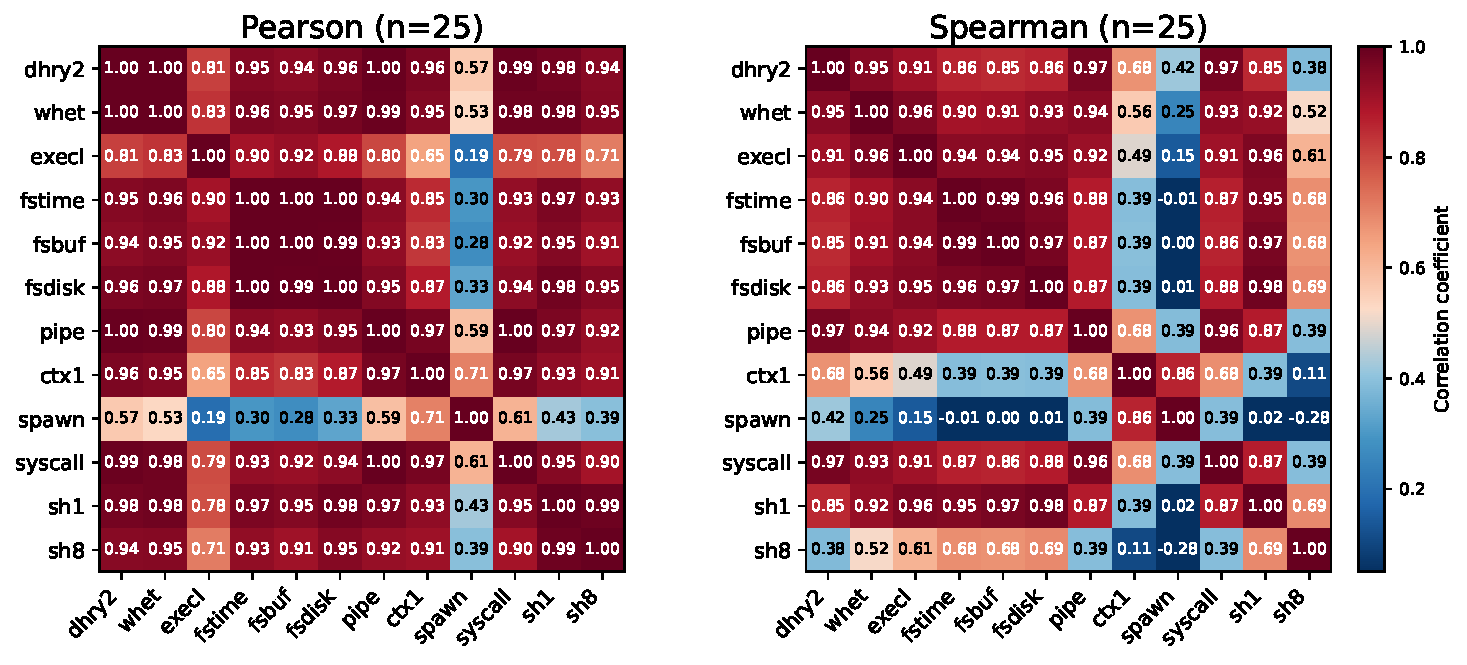
\includegraphics[width=1\linewidth]{images/unixbench_subtest_correlation_combined.pdf}
    \caption{Pairwise UnixBench subtest score correlation on five heterogeneous hosts ($n{=}25$ single-copy runs).
    Left: Pearson $r$; right: Spearman $\rho$.
    Dark red marks redundant pairs; lighter cells indicate weaker coupling for complementary Top-$K$ selection.}
    \label{fig:unixbench-subtest-correlation}
\end{figure}
The heatmaps show dense CPU clusters with $r{\ge}0.99$ among \id{dhry2reg}, \id{whetstone-double}, \id{pipe}, and \id{syscall}, and equally tight filesystem clusters among \id{fstime}, \id{fsbuffer}, and \id{fsdisk}.
Cross-cluster coupling is weaker: \id{spawn} versus filesystem tests yields $r{\approx}0.2$--$0.3$.
This structure justifies selecting $K{\ll}N$ diverse experts and reconstructing correlated components rather than executing all $N$ subtests.


\paragraph{Insight 2: Performance Metrics Exhibit Early Convergence.}
\label{subsec:motivation-convergence}
When full-suite execution is unavoidable, traditional methodologies mandate a rigid run-to-completion model.
However, many benchmark components are fundamentally iterative rate tests: the Dhrystone and Whetstone components in UnixBench~\cite{smith2011byte} continuously execute integer and floating-point kernels over a prolonged loop and report an accumulated operation rate in operations per second.
On our testbeds, the prefix rate sampled at 0.5\,s intervals typically stabilizes within the first 4--8\,s of execution, while official UnixBench components may run for minutes.
Continuing the workload to its official timeout primarily reduces statistical variance rather than altering the fundamental performance metric.
This gap between convergence time and protocol time motivates vertical cost reduction via aggressive, time-bounded probing (Section~\ref{subsec:time-bounded-probing}).

\paragraph{Insight 3: Production Telemetry is Inherently Fragile.}
Short probes and eBPF/PMU tracing routinely encounter timeouts, permission denials, and missing counters on shared cloud hosts.
Hypervisors may block \texttt{perf} event groups; tenant isolation may disable bpftrace; and heavy neighbor load can prevent a 4\,s micro-probe from reaching a steady rate.
A deployable toolchain must record these conditions---timeout flags, tracer-availability bits, elapsed wall time---as first-class features and continue inference rather than discard runs as statistical outliers.
This requirement shapes both feature collection (Section~\ref{subsec:feature-collection}) and probe training (Section~\ref{subsec:time-bounded-probing}).




\section{Methods}
\label{sec:methods}

\begin{figure}
    \centering
    \includegraphics[width=1\linewidth]{images/mob.pdf}
    \caption{Overview of the \ourmethod architecture. (1)~\textbf{Host OS:} collector aggregates static and dynamic metrics into $\mathbf{x}$. (2)~\textbf{Router:} scores experts and selects Top-$K$. (3)~\textbf{Probing:} category micro-workloads (or real subtests) run under a fixed budget and emit $\mathbf{p}$. (4)~\textbf{Reconstructor:} multi-output regressor predicts $\hat{\mathbf{y}}$ and $\hat{Y}$; an optional uncertainty head estimates per-target $\sigma$ (Section~\ref{subsec:uncertainty-estimator}) but is \emph{not} used in the default single-pass pipeline.}
    \label{fig:mob}
\end{figure}


\subsection{Overview}
\label{subsec:method-overview}

\ourmethod approximates a complete benchmark run by observing only a small subset of informative sub-benchmarks (Figure~\ref{fig:mob}; scope in Section~\ref{subsec:problem-scope}). 
Given target system state, it collects context \(\mathbf{x}\), routes Top-$K$ subtests, runs fixed-duration probes on the selected components, and reconstructs the full official profile (Sections~\ref{subsec:router}--\ref{subsec:reconstructor}).
The pipeline is \emph{single-pass}: budgets ($K$, probe duration) are fixed at deployment time---there is no adaptive re-probing loop.

\paragraph{End-to-end data flow.}
\textbf{Offline (per host $h$):} collect $M$ complete suite runs $\{(\mathbf{x}_i,\mathbf{y}_i,Y_i)\}_{i=1}^M$ with official per-component scores $\mathbf{y}_i$ and suite index $Y_i$.
Train (1) router $f_\theta$ from $(\mathbf{x}_i,\mathbf{y}_i)$, (2) probe estimators $f_{e_j}$ from prefix telemetry $(\mathbf{p}_{i,j},y_{i,j})$ for each expert $e_j$, and (3) reconstructor $g_\phi$ from masked partial vectors and full labels.
\textbf{Online (new run on $h$):} collect $\mathbf{x}$ $\rightarrow$ select $\mathcal{S}_K(\mathbf{x})$ $\rightarrow$ for each selected expert $e_j\in\mathcal{S}_K$, execute one bounded probe and predict $\hat{y}_j=f_{e_j}(\mathbf{p}_j)$ $\rightarrow$ form sparse tuple $Z=[\mathbf{x},m_j,\hat{y}_j,\tau_j]$ $\rightarrow$ output $\hat{\mathbf{y}},\hat{Y}=g_\phi(Z)$, where $m_j$ is the observation mask and $\tau_j$ is probe wall time.
Error propagates sequentially: probe error on the $K$ observed components is absorbed by $g_\phi$ when imputing unobserved $y_j$ and the aggregate $Y$; we do not re-route or extend probes based on posterior uncertainty.

\paragraph{Online execution protocol.}
On a target host, \ourmethod executes four deterministic stages without adaptive re-probing.
(1)~\textbf{Profile:} collect $\mathbf{x}$ with a 3\,s warmup, 0.5\,s \path{/proc} sampling, and perf PMU counters when permitted; if PMU access is blocked, the collector records a degradation flag and continues with \path{/proc}-only proxies.
(2)~\textbf{Route:} score every expert $e_j\in\mathcal{E}$ with $f_\theta$ and select $\mathcal{S}_K(\mathbf{x})$.
(3)~\textbf{Probe:} for each $e_j\in\mathcal{S}_K$, launch one micro-probe (default $T_{\mathrm{probe}}{=}4$\,s), collect $\mathbf{p}_j$, and predict $\hat{y}_j$.
(4)~\textbf{Reconstruct:} assemble $Z$ and emit all component scores $\hat{\mathbf{y}}$ plus the official suite index $\hat{Y}=A(\hat{\mathbf{y}})$.
Default wall time is $T_{\mathbf{x}}+K{\cdot}T_{\mathrm{probe}}$ (${\approx}15$\,s for $K{=}3$), versus $C_{\mathrm{full}}$ in Equation~\ref{eq:full-cost}.
All models are trained and deployed per host so $\mathbf{x}$, probes, and labels share the same telemetry semantics at inference time.

\paragraph{Systems contribution beyond score regression.}
Execution-free predictors~\cite{wang2019predicting,tousi2022comparative} map static host descriptors to suite scores without measuring the target machine under contention.
\ourmethod instead defines a \emph{bounded measurement protocol}: sparse real workloads, live /proc/perf/eBPF telemetry with explicit degradation paths, official suite aggregation $A(\cdot)$, and per-host model training.
The contribution is therefore jointly algorithmic (conditional Top-$K$ selection plus reconstruction from sparse observations) and systems-oriented (predictable $T_{\mathrm{partial}}$, timeout/missing-tracer encoding, and deployability on restricted cloud kernels), rather than improving offline regression $R^2$ on a static feature table alone.

\begin{table*}[t]
\centering
\caption{Purpose-oriented feature groups organized by collection stage. Pre-run signals form the system context \(\mathbf{x}_i\), while in-run probe signals form the probe vector \(\mathbf{p}_{i,j}\).}
\label{tab:feature_collection}
\small
\setlength{\tabcolsep}{5pt}
\renewcommand{\arraystretch}{1.10}
\begin{tabular}{p{0.08\linewidth}| p{0.17\linewidth} p{0.27\linewidth} p{0.42\linewidth}}
\toprule
\textbf{Stage} & \textbf{Signal type} & \textbf{Purpose} & \textbf{Representative signals} \\
\midrule

\multirow{3}{=}{Pre-run}
& Static host profile
& Identify stable host configuration.
& CPU topology, NUMA layout, memory size, compiler versions \\

& System pressure
& Capture transient pre-run load.
& CPU/GPU utilization, iowait, load average, runnable tasks \\

& PMU / perf
& Characterize microarchitectural behavior.
& IPC, cycles/s, instructions/s, cache/branch miss ratios \\

\midrule

\multirow{5}{=}{In-run}
& Probe progress
& Record observed benchmark progress.
& Configured probing duration, elapsed wall-clock time \\

& eBPF-based tracing
& Observe prefix-level kernel activity.
& Scheduling-switch rate, syscall-entry rate, eBPF availability \\

& Resource usage
& Summarize prefix resource usage.
& User/system/idle CPU ratio, minor faults, major faults \\

& Workload identity
& Provide workload semantic context.
& CPU, memory, I/O, thread, syscall, GPU category \\

& Probe flags
& Mark probe mode and failures.
& Micro workload flag, real-component flag, timeout flag \\

\bottomrule
\end{tabular}
\end{table*}

\subsection{Feature Collection and Engineering}
\label{subsec:feature-collection}

Feature collection provides the contextual information required to reduce benchmark cost while preserving the ability to estimate full-suite performance. The framework observes three factors that affect measured performance: what the machine is, what state the machine is in, and how a benchmark behaves.

For the $i$-th benchmark run, we define the system context vector as
\begin{equation}
\label{eq:system-context}
\mathbf{x}_i = [\mathbf{x}_i^{\mathrm{static}}, \mathbf{x}_i^{\mathrm{dynamic}}]
\end{equation}
where $\mathbf{x}_i^{\mathrm{static}}$ covers stable host descriptors---CPU topology, total memory, OS and compiler versions---and $\mathbf{x}_i^{\mathrm{dynamic}}$ captures pre-run transient state---system load, runnable-task counts, and hardware-counter snapshots from perf or \path{/proc}.
The vector $\mathbf{x}_i$ is collected once before a full-suite run and is consumed by both the router and the probe estimators.

During short-run probing, the framework further collects a probe-specific vector $\mathbf{p}_{i,j}$ for benchmark component $b_j$. Unlike $\mathbf{x}_i$, which describes the global context of the $i$-th run, $\mathbf{p}_{i,j}$ summarizes the execution prefix of a specific component, capturing wall-clock time, context-switch rates, and categorical identifiers. Table~\ref{tab:feature_collection} summarizes these feature groups by collection stage and purpose.

\paragraph{Feature Processing and Domain-Aware Scaling.}
Raw system telemetry cannot be directly fed into the models.
Global MinMax or z-score normalization obscures physical limits across heterogeneous machines; \ourmethod instead employs domain-aware semantic scaling.
Static capacities (total CPU cores, memory in GiB) keep physical magnitudes so the model sees each host's ceiling.
Dynamic metrics become ratios or rates: CPU utilization and I/O wait map to percentages; monotonic counters (page faults, context switches, PMU instructions) convert to per-second rates.
Workload-type and probe-failure indicators use one-hot encoding.
All missing values are zero-filled to maintain a deterministic tensor shape for inference.

\paragraph{Cost-Aware Collection and Fallbacks.}
Extracting PMU (Performance Monitoring Unit) events and eBPF traces incurs overhead and relies on specific kernel configurations. Rather than statistically pruning these informative features, \ourmethod adopts an engineering-driven fallback strategy to balance extraction cost and prediction accuracy. If high-overhead \texttt{perf} counters are unavailable or blocked by the hypervisor, the collector safely degrades to standard \texttt{/proc} statistics. Similarly, if eBPF tracing is disabled or GPU telemetry is absent on CPU-only instances, the framework zero-masks the corresponding vector dimensions. This robust collection pipeline ensures that the benchmarking methodology remains lightweight and executable across strictly isolated cloud tenants or bare-metal machines.


\subsection{Router: Conditional Expert Selection}
\label{subsec:router}

A full benchmark suite contains inherent redundancy. Although each sub-benchmark targets a specific subsystem, their outputs are jointly determined by the underlying system state, including CPU throughput, memory hierarchy behavior, operating-system overhead, and scheduler effects.
In UnixBench, \id{dhry2reg} and \id{whetstone-double} reflect computation capability, while \id{pipe} and \id{syscall} capture OS-level overheads.
Because these sub-benchmarks provide different projections of the same system configuration, a carefully selected subset can retain sufficient information for reconstructing the full-suite profile.

The informative subset, however, is not fixed across systems. A CPU-bound system state may require different probes than an I/O- or OS-overhead-bound state. \ourmethod therefore formulates benchmark acceleration as a conditional expert selection problem: given a current system feature vector \(\mathbf{x}\), the router selects a small set of sub-benchmarks whose measurements are expected to be most useful for reconstructing the full-suite result.

\paragraph{Expert Routing.}
We treat each independently executable sub-benchmark as a measurement expert in a fixed pool:
\begin{equation}
\label{eq:expert-pool}
\mathcal{E}=\{e_1,e_2,\ldots,e_n\}.
\end{equation}
Each expert \(e_i\) corresponds to a sub-benchmark identifier and optional metadata including historical execution cost. Before execution, the router only observes the system feature vector and expert metadata; after execution, expert \(e_i\) returns a measured score \(r_i\) and incurs cost \(c_i\).

Routing is not a standard multi-class classification problem, because the goal is not to assign each system state to a single best benchmark. Instead, the router must estimate the conditional utility of every candidate expert and select a subset. Given \(\mathbf{x}\), a scoring model \(f_\theta\) assigns each expert a relevance score:
\begin{equation}
\label{eq:router-score}
s_i=f_\theta(\mathbf{x},e_i).
\end{equation}
The scores are normalized into selection probabilities:
\begin{equation}
\label{eq:router-prob}
p_i=\frac{\exp(s_i)}{\sum_{j=1}^{n}\exp(s_j)}.
\end{equation}
The router then executes the Top-\(K\) experts:
\begin{equation}
\label{eq:topk}
\mathcal{S}_K(\mathbf{x})=\operatorname{TopK}_{e_i\in\mathcal{E}} p_i.
\end{equation}
The resulting partial observation vector is passed to the reconstructor to estimate the full-suite profile.

\paragraph{Training Objective.}
For each historical run $i$, we form one ranking query over the full expert pool $\mathcal{E}$: all experts share the same context $\mathbf{x}_i$, and expert $e_j$ receives label $y_{i,j}$, the official full-run component index from $\mathbf{y}_i$.
The LightGBM router minimizes a pairwise ranking loss over these query groups; neural routers minimize cross-entropy to the normalized label vector $\{y_{i,j}/\sum_k y_{i,k}\}$.
The goal is to rank conditionally informative experts, not to predict $Y$ directly---suite recovery is delegated to the reconstructor fed with probe-imputed partial scores.
At inference, only the Top-$K$ ranked experts are executed; unselected experts contribute mask bits but no observed scores to the reconstructor input.

\paragraph{Budget Control.}
The budget parameter \(K\) controls the accuracy--cost trade-off. Smaller \(K\) reduces execution time but provides fewer observations to the reconstructor, while larger \(K\) improves measurement coverage at higher cost.


\subsection{Time-Bounded Probing}
\label{subsec:time-bounded-probing}

In addition to reducing the number of executed sub-benchmarks, \ourmethod further reduces the evaluation cost of each selected expert through time-bounded probing. Instead of running an iterative sub-benchmark until its official loop completes, \ourmethod executes a short probe for a predefined time window and leverages the collected telemetry, calibrated against historical full-run labels, to estimate the full sub-benchmark score.

The probe duration is strictly clamped within a fixed and safe operational window to avoid runaway executions caused by anomalous inputs or unstable runtime behavior. \ourmethod does not repeatedly query a model to decide whether to halt. Instead, it enforces a hard wall-clock limit and uses a supervised estimator to map the truncated execution signature to the final benchmark score. This design converts an unpredictable benchmark execution into a bounded observation procedure with a controllable time budget.

\paragraph{Dual-Mode Probing: Micro and Real.}
\ourmethod supports \textbf{micro-probes} and \textbf{real-probes}.
Micro-probes map each selected expert $e_j$ to a coarse category (CPU, memory, I/O, syscall, thread, or GPU) and run a short synthetic stimulus for a fixed budget---for example, a tight sqrt loop for CPU experts such as \id{dhry2reg}, or repeated temp-file read/write for I/O experts such as \id{fstime}---while collecting eBPF/\path{/proc} telemetry.
Real-probes invoke the original subtest under a hard timeout and record the same telemetry channels when permitted.
Both modes emit the same interface: bounded telemetry $\mathbf{p}_{i,j}$ and predicted full-run score $\hat{y}_{i,j}$ against the official label $y_{i,j}$; only the observation stimulus differs.

\paragraph{Calibrated Micro-Probing for High-Cost Experts.}
Real probes match benchmark semantics but can incur large startup overhead; micro-probes replace the observation stimulus with a short category-level workload while the \emph{supervision target remains the official full-run score} of the original sub-benchmark.
Formally, for run $i$ and expert $e_j$, a micro-probe yields telemetry vector \(\mathbf{p}^{\mathrm{micro}}_{i,j}\) and the estimator learns:
\begin{equation}
\label{eq:probe-predict}
\hat{y}_{i,j} = f_{e_j}(\mathbf{p}^{\mathrm{micro}}_{i,j}),
\end{equation}
or, in the shared-estimator setting,
\begin{equation}
\label{eq:probe-predict-shared}
\hat{y}_{i,j} = f(\mathbf{p}^{\mathrm{micro}}_{i,j}, \mathrm{id}(e_j)),
\end{equation}
where $\mathrm{id}(e_j)$ one-hot-encodes expert identity and $y_{i,j}$ is the historical full-run label.
The reconstructor consumes only \(\hat{y}_{i,j}\), regardless of probe mode.

\paragraph{Engineering Robustness over Outlier Rejection.}
Unlike conventional machine learning pipelines that aggressively discard truncated executions, timeouts, or noisy runs as statistical outliers, \ourmethod treats these execution anomalies as measurable system states when they arise from the bounded probing procedure. In production environments, telemetry collection can be imperfect due to permission restrictions, missing tracing tools, or heavy system load. \ourmethod therefore encodes such conditions explicitly rather than terminating the evaluation pipeline.

\begin{itemize}
    \item \textbf{Encoding Truncation as Features:} If a real probe is killed by the timeout, the event is not discarded. Instead, \id{real\_timed\_out}, \id{workload\_rc}, and elapsed wall-clock time are explicitly encoded into the feature vector so the estimator can interpret forcefully truncated runs.
    \item \textbf{Graceful Degradation for eBPF:} If high-fidelity eBPF tracing is unavailable due to kernel restrictions, missing tools, or insufficient privileges, the framework does not crash. It records \id{ebpf\_available}${=}0$ and zero-masks the corresponding eBPF dimensions, allowing the estimator to fall back on standard \path{/proc} counters and other available system features.
    \item \textbf{Rate Conversion:} To ensure telemetry is comparable across probes with slightly different elapsed durations, monotonically increasing eBPF counters (\id{sched\_switch}, \id{syscall\_enter}) are converted to per-second rates before vectorization.
\end{itemize}

\paragraph{Training objective and inference.}
Each probe sample pairs prefix telemetry $\mathbf{p}_{i,j}$ with full-run label $y_{i,j}$ from the same historical run.
The estimator minimizes squared error in label space---official UnixBench indices for UB, $\log(1+y)$-transformed PTS primaries for PTS---$\mathcal{L}_{\mathrm{probe}}=\sum_{i,j}(\hat{y}_{i,j}-y_{i,j})^2$, with invalid labels filtered at dataset construction.
At inference, one bounded probe on expert $e_j$ produces $\mathbf{p}_j$ and $\hat{y}_j=f_{e_j}(\mathbf{p}_j)$ in official benchmark units after inverse scaling.
This replaces unpredictable run-to-completion cost with fixed $T_{\mathrm{probe}}$.


\subsection{Reconstructor: Full-Suite Result Recovery}
\label{subsec:reconstructor}

After the router selects and executes a small subset of sub-benchmarks, \ourmethod relies on a reconstructor to recover the full benchmark outcome. The reconstructor addresses the sparse observation problem: given the current system feature vector and the partial subtest results, it acts as a multi-output regression model to simultaneously predict the scores of all unexecuted sub-benchmarks as well as the aggregate suite score.

\begin{figure}
    \centering
    \includegraphics[width=1\linewidth]{images/recontruct.pdf}
    \caption{Reconstructor training with random-masked full runs. Historical full-run results are randomly masked to generate augmented sparse samples. The reconstructor takes the masked scores and binary mask as input, predicts the full-run result, and is optimized using the original full-run result as the supervision target.}
    \label{fig:reconstructor-training}
\end{figure}

\paragraph{Input Representation and Multi-Output Target.}
To make sparse benchmark results consumable by a fixed-size tensor, \ourmethod encodes all experts $e_1,\ldots,e_n$ in a canonical order aligned with $\mathcal{E}$.
Each expert $e_i$ is represented by a 3-tuple \(z_i = (m_i, v_i, \tau_i)\), where \(m_i \in \{0,1\}\) is a binary observation mask, \(v_i\) is the observed or probe-predicted score when $e_i$ is selected, and \(\tau_i\) is the corresponding probe wall time.
For unexecuted experts, the tuple is zero-filled.
The final input vector concatenates the system context \(x\) with the masked partial observations:
\begin{equation}
\label{eq:recon-input}
X = [x,\, m_1, v_1, \tau_1,\, \ldots,\, m_n, v_n, \tau_n]
\end{equation}
The output target is the complete benchmark profile derived from historical full runs: \(Y = [r_1, r_2, \ldots, r_n, S]\), where \(S\) is the final reported index.
For tree-based models (LightGBM and XGBoost), \ourmethod wraps the base regressor with a multi-output strategy to train an independent regressor per target dimension.

\paragraph{Training via simulated sparse execution.}
Because historical data contain only complete runs, training augments each $(\mathbf{x}_i,\mathbf{y}_i,Y_i)$ into multiple masked samples (Figure~\ref{fig:reconstructor-training}): sample $k\in[k_{\min},k_{\max}]$, mask unexecuted components in $Z$, and supervise with the full target $Y_i$ and all $y_{i,j}$.
The reconstructor minimizes per-dimension squared error, $\mathcal{L}_{\mathrm{recon}}=\|\hat{\mathbf{y}}-\mathbf{y}\|^2+(\hat{Y}-Y)^2$, over augmented masks so it generalizes to router-chosen sparsity patterns at inference.

\paragraph{Official aggregator $A(\cdot)$ across suites.}
\label{subsec:aggregator}
\ourmethod never invents a surrogate suite metric: training labels and evaluation references always follow each framework's official semantics.
\textbf{UnixBench:} component labels $y_{i,j}$ are per-subtest \emph{Index} scores from the run JSON; the suite label $Y$ is the published \emph{System Benchmarks Index Score} (\texttt{system\_benchmarks\_index\_score}), i.e., UnixBench's own $A(\mathbf{y})$, not recomputed from components at label time.
\textbf{PTS:} each profile reports a primary throughput/latency value $v_j$; when a profile emits multiple result blocks, we reduce them with the same log-mean used for suite aggregation:
\begin{equation}
\label{eq:pts-logmean}
A_{\mathrm{logmean}}(\mathbf{v})=\exp\!\left(\tfrac{1}{N}\sum_{j=1}^{N}\log(1+v_j)\right)-1.
\end{equation}
The reconstructor's last output dimension is supervised with this $Y$ (UnixBench: official index; PTS: $A_{\mathrm{logmean}}$ over profile primaries).
\textbf{Probe-only path:} when all components are probe-predicted without reconstruction, UnixBench suite scores use the same geometric-mean-over-indices rule $A_{\mathrm{geomean}}(\hat{\mathbf{y}})=\exp(\mathrm{mean}_j(\log(1+\hat{y}_j))-1$.

\paragraph{Scale compression for heterogeneous targets.}
PTS profile primaries span orders of magnitude; probe estimators therefore train in $\log(1+y)$ space and apply \texttt{expm1} at inference.
Reconstructor training applies $\log(1+\cdot)$ to \emph{partial} UnixBench index inputs and to all PTS partial values when building $Z$, while still supervising the suite dimension with the official $Y$ above.
This keeps per-component and suite targets on comparable scales without per-profile instance weighting.

\paragraph{Uncertainty estimator (Figure~\ref{fig:mob}).}
\label{subsec:uncertainty-estimator}
Figure~\ref{fig:mob} shows an optional uncertainty head attached to the reconstructor.
It is exported with v2 model bundles but \emph{not} consulted in the evaluated single-pass Hybrid pipeline (fixed $K$, no adaptive re-probing; Section~\ref{subsec:method-overview}).
\textbf{Tree reconstructors (LightGBM/XGBoost):} after fitting the main multi-output regressor, a secondary multi-output model predicts the absolute training residual $|\hat{y}^{(k)}-y^{(k)}|$ per target dimension $k$ (including the suite index); at inference $\sigma_k$ is this residual model's output, used as a heteroscedasticity proxy.
\textbf{MLP reconstructor:} a twin-head network minimizes Gaussian negative log-likelihood with per-target mean and $\log$-variance outputs; $\sigma_k=\exp(\tfrac{1}{2}\log v_k)$.
The estimator exposes $\sigma^{\mathrm{suite}}$ and per-expert $\sigma_j$; $1/(1+\sigma^{\mathrm{suite}})$ is reported as a confidence proxy.
An optional active-refinement mode (not evaluated in Table~\ref{tab:overall-effectiveness-expanded}) could probe the unexecuted expert with largest $\sigma_j$, but our production protocol stops after the router's Top-$K$ budget.



\section{Evaluation}
\label{sec:evaluation}

\subsection{Experimental Setup}
\label{subsec:exp-setup}

% We evaluate \appname{} on five heterogeneous Linux hosts.
% UnixBench and \ptscpu{} run on all five machines; \ptsgpu{} runs on H1 only.

% Our primary method is the integrated Hybrid pipeline.
% We collect $\mathbf{x}$ once, use a router to select Top-$K$ sub-benchmarks, run a short probe (default 4\,s) on \emph{only} those selected components, and reconstruct the full-suite score from probe-predicted partial observations.
% Ground-truth scores and wall times come from previously collected complete runs on the same host (offline replay); we do \emph{not} re-execute full suites during hybrid evaluation.

% We exhaustively compare all $3 \times 2 \times 3 = 18$ router--probe--reconstructor combinations on each applicable host--suite pair.
% \emph{Router only} (Top-$K$ \emph{full} partial execution + reconstruction) and \emph{probe only} (probe \emph{all} components without reconstruction) are retained as ablation baselines.
% Unless stated otherwise, each host trains and evaluates only on its own collected runs.

% Main-experiment and supplementary tables report measured means over five hosts (or H1 only for \ptsgpu{}).
% Values are aggregated from per-host offline cross-validation JSON under \path{dataset/paper_supplementary/}.

% \subsubsection{Testbeds}
% \label{subsubsec:testbeds}
\paragraph{Hardware environment.}

We deploy \appname{} on five heterogeneous Linux hosts (Table~\ref{tab:testbeds}).
H1 (32 vCPUs, Intel Core i9-14900K, 128\,GiB RAM, NVIDIA RTX 3090 Ti GPU) is the development server and sole \ptsgpu{} host; H2--H5 are smaller CPU-only cloud instances (Intel Xeon 6982P-C or Xeon Platinum) for UnixBench and \ptscpu{}.
All machines share Ubuntu 22.04.5 LTS and GCC 11.5.0; H1 additionally uses NVIDIA driver 580.159.03, PyTorch 2.12.0+cu130, and TensorFlow 2.21.0.
We label hosts by a compact CPU$\times$RAM shorthand used throughout this section.


\begin{table}[t]
\centering
\caption{Evaluation testbeds. Five Linux hosts with heterogeneous CPU and memory capacity. CPU models are taken from \path{/proc/cpuinfo} at collection time. \ptsgpu{} runs only on H1.}
\label{tab:testbeds}
\small
\setlength{\tabcolsep}{4pt}
\begin{tabular}{@{}lp{0.36\linewidth}rc@{}}
\toprule
\textbf{Host} & \textbf{vCPU (CPU model)} & \textbf{RAM} & \textbf{GPU} \\
\midrule
H1 & 32 (Intel Core i9-14900K) & 128GB & NVIDIA RTX 3090 Ti GPU \\
H2 & 2 (Intel Xeon 6982P-C) & 8GB & --- \\
H3 & 4 (Intel Xeon 6982P-C) & 8GB & --- \\
H4 & 4 (Intel Xeon 6982P-C) & 16GB & --- \\
H5 & 8 (Intel Xeon Platinum) & 8GB & --- \\
\bottomrule
\end{tabular}
\end{table}


\paragraph{Software environment.}
Each host runs a Linux kernel with standard perf and optional bpftrace support.
System feature collection (\(\mathbf{x}\)) uses a 3\,s warmup, 0.5\,s \path{/proc} sampling, and a 64\,MiB in-process warmup working set unless noted otherwise.
When perf PMU counters are blocked, the collector falls back to \path{/proc}-based proxies without aborting the pipeline.
On H1, NVIDIA driver and OpenCL inventory are collected when available; on CPU-only hosts (H2--H5), GPU dimensions are zero-masked at inference.



\paragraph{Benchmark Suites}
\label{subsubsec:benchmark-suites}

We evaluate on three benchmark suites that stress complementary subsystems.
UnixBench and \ptscpu{} are run on all five hosts; \ptsgpu{} is restricted to H1 because the other four machines lack discrete GPUs.

\begin{itemize}
    \item \textbf{UnixBench (UB).} A classic system-level suite with 12 single-copy subtests (\(N=12\)): \id{dhry2reg}, \id{whetstone-double}, \id{execl}, \id{fstime}, \id{fsbuffer}, \id{fsdisk}, \id{pipe}, \id{context1}, \id{spawn}, \id{syscall}, \id{shell1}, and \id{shell8}.
    The suite spans CPU kernels, filesystem I/O, and OS/interaction workloads.
    We run UnixBench with a single parallel copy (\id{perl Run -c 1}), matching the \appname{} collection protocol.
    The aggregate metric is the \emph{System Benchmarks Index Score}.

    \item \textbf{Phoronix Test Suite --- CPU (\ptscpu).} The standard CPU suite with approximately 13 profiles spanning compilation (\id{build-linux-kernel}), cryptography, compression, and numerical kernels.
    Each profile reports a primary throughput or latency metric; suite aggregation follows log-mean over profiles, consistent with our reconstructor training target.

    \item \textbf{Phoronix Test Suite --- GPU (\ptsgpu).} The NVIDIA GPU compute suite, executed only on H1, which has a suitable NVIDIA GPU and installed PTS profiles.
    This suite complements CPU-centric evaluation with OpenCL/GPU compute workloads and is omitted on H2--H5.
\end{itemize}

On each host, we collect multiple complete benchmark sessions (typically 3--5 rounds per session) for every suite applicable to that host.

\paragraph{Why UnixBench and PTS, not SPEC CPU2017.}
SPEC CPU2017 is the industrial processor reference, but our target workflows---cloud auto-tuning, regression testing, and operator monitoring---need open, scriptable suites that exercise CPU, I/O, OS, and GPU subsystems without license-managed publication.
We evaluate on UnixBench and PTS accordingly; certified SPEC submission lies outside our scope (Section~\ref{subsec:problem-scope}).

\paragraph{Baselines.}
We compare \ourmethod against three baselines.
The \emph{full-run} baseline executes the entire suite and provides the reference result with no runtime reduction.
Wang et al.~\cite{wang2019predicting} train a deep neural network to predict processor benchmark scores from public CPU specifications and historical benchmark tables.
Tousi et al.~\cite{tousi2022comparative} study supervised regression for predicting SPEC CPU2017 results from hardware and software configurations---representative of industrial-grade, execution-free SPEC prediction pipelines.
We include Tousi et al.\ to test whether SPEC-trained models transfer to UnixBench and PTS on the same hosts.
Both execution-free baselines use leave-one-run-out cross-validation; wall time is $\mathbf{x}$ collection only ($\approx$3.5\,s).
Unlike these prediction-only baselines, \ourmethod selectively runs a small subset of experts and reconstructs the full-suite result from bounded on-host probes.
All methods share the same train/test splits whenever the required input features are available.

\paragraph{Evaluation organization.}
The remainder of Section~\ref{sec:evaluation} is organized around three execution paths.
\textbf{(1)~Hybrid pipeline (\ourmethod{} main method):}
collect $\mathbf{x}$, router Top-$K$, micro-probe selected components, reconstruct the suite score (router $\rightarrow$ probe $\rightarrow$ reconstruct).
We first report five-host end-to-end effectiveness (Section~\ref{subsec:overall-effectiveness}), followed by a runtime overhead analysis using UnixBench resource waveforms (Section~\ref{subsec:resource-waveforms}).
\textbf{(2)~\emph{Router only} ablation:}
replace probe predictions with \emph{measured} partial sub-benchmark scores on the router-selected subset, then reconstruct (Section~\ref{subsec:model-combination}), with supplementary offline studies on Top-$K$ and system-feature ablation (Sections~\ref{subsec:topk-tradeoff},~\ref{subsec:feature-ablation}).
\textbf{(3)~\emph{Probe only} ablation:}
probe every component without router selection or reconstruction (Section~\ref{subsec:probe-evaluation}).

\paragraph{Hybrid evaluation protocol.}
Table~\ref{tab:overall-effectiveness-expanded} reports the primary Hybrid path (router $\rightarrow$ probe $\rightarrow$ reconstruct).
For each historical run, we replay only the pre-run context $\mathbf{x}$ and the probe telemetry $\mathbf{p}$ from prior micro-probes on that run; the router, probe estimators, and reconstructor then produce $\hat{\mathbf{y}}$ and $\hat{Y}$.
The reconstructor input contains \emph{probe-imputed} scores $\hat{y}_j$ on the router-selected subset---never measured partial subtest scores from the full-run JSON.
We compare $\hat{Y}$ against the reference full-suite index $Y$ from the same run solely to compute error.
This offline protocol avoids re-executing thousand-second full suites during cross-validation; Section~\ref{subsec:resource-waveforms} corroborates wall-time savings with online traces.
\emph{Router only} ablations (Sections~\ref{subsec:model-combination}--\ref{subsec:feature-ablation}) deliberately substitute \emph{measured} partial scores to isolate routing and reconstruction; their higher errors (0.1--2\%) must not be conflated with Hybrid headline numbers.

% \paragraph{Per-host training protocol.}
% For every host from H1 to H5, we collect benchmark datasets locally and train all models using only runs whose session tags match that host.
% H1 trains and evaluates on UnixBench, \ptscpu, and \ptsgpu; H2--H5 train and evaluate on UnixBench and \ptscpu{} only.
% This isolates each machine's router, reconstructor, and probe models from other hosts' data distributions.
% Cross-host comparison therefore reflects how \appname{} behaves under different hardware ceilings rather than a single global model transferred across machines.


% For hybrid and \emph{router only} end-to-end grid experiments on PTS, ground-truth full-suite scores are taken from previously collected full runs on the same host (offline replay), avoiding repeated full-suite online execution that can cause excessive wall time or resource exhaustion.
% Hybrid UnixBench evaluation likewise replays historical runs for accuracy and uses dataset-recorded full-suite wall times for cost comparison.

% \subsubsection{Collected Data}
% \label{subsubsec:collected-data}

% \paragraph{Phase~1: Full-suite collection (shared by all routes).}
% On each host, we collect multiple complete benchmark sessions (typically 3--5 rounds per session) for every suite applicable to that host.
% UnixBench and \ptscpu{} sessions are collected on all five hosts; \ptsgpu{} sessions are collected on H1 only.
% Each run record stores system context $\mathbf{x}$, per-component results $\mathbf{y}$ and timings $\mathbf{t}$, and expert metadata (component identifiers, categories, and titles).
% These runs provide supervision for router training, reconstructor training, probe label construction, and ground-truth evaluation.

% \paragraph{Phase~2: Hybrid main experiment (router + probe + reconstruct).}
% For each applicable suite on each host, we train three router architectures (LightGBM ranker, MLP, GNN-expert), three reconstructors (XGBoost, LightGBM, MLP), and two probe regressors (LightGBM and XGBoost).
% We evaluate all $3 \times 2 \times 3 = 18$ hybrid combinations offline.
% For each historical run, the router selects Top-$K$ components, probe predictions substitute for executed subtest scores on the selected subset only, and the reconstructor predicts the suite score.
% Partial wall time is estimated as $\hat{T}_{\mathrm{xi}} + K \cdot T_{\mathrm{probe}}$ (default $\hat{T}_{\mathrm{xi}}=3$\,s, $T_{\mathrm{probe}}=4$\,s); full-suite wall time is read from the dataset.

% \paragraph{Phase~3: Ablation --- \emph{router only} (partial full execution + reconstruction).}
% We repeat the \(3 \times 3\) router--reconstructor grid using \emph{actual} partial sub-benchmark execution scores (not probe predictions) on the router-selected subset, matching the original \emph{router only} design.

% \paragraph{Phase~4: Ablation --- \emph{probe only} (probe all components).}
% For each applicable suite on each host, we build a probe dataset by executing short probes (default 4\,s per component, micro-probe mode) over historical full runs on the same host, train two regressors (LightGBM and XGBoost), and evaluate suite prediction by probing \emph{every} component and aggregating---without router selection or reconstruction.

% \paragraph{Phase~5: Supplementary offline studies (\emph{router only} best combination).}
% After selecting the best router--reconstructor pair per suite from Phase~2 on each applicable host, we conduct three supplementary studies on stored runs only (leave-one-session-out cross-validation, no re-execution):
% Top-$K$ sweep, routing-policy comparison, and system-feature ablation.
% For \ptsgpu, supplementary studies use H1 data only.


% \subsection{Data Collection and Training Protocol}
% \label{subsec:data-and-protocol}

% To ensure rigorous evaluation and prevent data leakage across heterogeneous hardware environments, we enforce a strict per-host protocol for both data collection and model training.

% \paragraph{Full-Suite Data Collection.}
% For every host from H1 to H5, we construct a local ground-truth dataset by executing multiple complete benchmark sessions (typically 3--5 full rounds per session) for every suite applicable to that host.
% Specifically, UnixBench and \ptscpu{} sessions are collected across all five machines, while \ptsgpu{} sessions are collected exclusively on H1.
% During each full-suite execution, the system records a comprehensive profile containing the pre-run system context $\mathbf{x}$, per-component score results $\mathbf{y}$, component execution timings $\mathbf{t}$, and associated expert metadata (e.g., component identifiers and workload categories).
% These complete historical runs serve as the foundational dataset, providing necessary supervision for router training, reconstructor targets, probe label construction, and final ground-truth evaluation.

% \paragraph{Per-Host Training Isolation.}
% We treat each machine as an independent operational environment.
% For every host, all models (including routers, reconstructors, and probe estimators) are trained using \emph{only} the runs whose session tags match that specific host.
% This design strictly isolates each machine's pipeline from the data distributions of others.
% Consequently, our cross-host evaluation reflects how \appname{} adapts to different hardware ceilings autonomously, rather than relying on a single, globally transferred model.

% \paragraph{Offline Replay for Evaluation.}
% Evaluating large-scale, comprehensive suites via repeated online execution incurs excessive wall-clock time and introduces unmanageable resource exhaustion and thermal throttling variances.
% To mitigate this, our end-to-end evaluations (including the Hybrid pipeline and ablation grids) adopt an offline replay methodology.
% For both PTS and UnixBench experiments, ground-truth full-suite scores and wall times are extracted directly from the previously collected datasets.
% During validation, the system simulates the partial execution by retrieving the corresponding sub-benchmark records, ensuring a statistically sound and highly reproducible cost comparison without the overhead of redundant physical executions.

\paragraph{Metrics and Evaluation Criteria}
\label{subsubsec:metrics}
We evaluate our methodology and summarize the results across testbeds using the following key metrics and aggregation strategies:
\begin{table*}[t]
\centering
\caption{Overall effectiveness across five heterogeneous hosts.
\ourmethod{} rows use the Hybrid pipeline: router Top-$K$, \emph{probe-model-predicted} partial scores, and reconstruction (Section~\ref{subsec:overall-effectiveness}).
Wang/Tousi rows are execution-free MLP proxies~\cite{wang2019predicting,tousi2022comparative} (static hardware features only).
Execution time is in seconds; lower is better for error and time. Bold marks best among tested methods.}
\label{tab:overall-effectiveness-expanded}
\footnotesize
\setlength{\tabcolsep}{4.5pt}
\begin{tabular}{llcccccccccc}
\toprule
\multirow{2}{*}{\textbf{Suite}} & \multirow{2}{*}{\textbf{Method}} & \multicolumn{2}{c}{\textbf{M1 (32U128G)}} & \multicolumn{2}{c}{\textbf{M2 (2U8G)}} & \multicolumn{2}{c}{\textbf{M3 (4U8G)}} & \multicolumn{2}{c}{\textbf{M4 (4U16G)}} & \multicolumn{2}{c}{\textbf{M5 (8U8G)}} \\
\cmidrule(lr){3-4} \cmidrule(lr){5-6} \cmidrule(lr){7-8} \cmidrule(lr){9-10} \cmidrule(lr){11-12}
& & \textbf{Err. (\%)} & \textbf{Time (s)} & \textbf{Err. (\%)} & \textbf{Time (s)} & \textbf{Err. (\%)} & \textbf{Time (s)} & \textbf{Err. (\%)} & \textbf{Time (s)} & \textbf{Err. (\%)} & \textbf{Time (s)} \\
\midrule

\multirow{4}{*}{UnixBench} 
& Full-suite & -- & 1691.0 & -- & 1520.0 & -- & 1580.0 & -- & 1610.0 & -- & 1550.0 \\
& Wang (MLP) & 0.21 & 3.5 & 2.67 & 3.5 & 6.28 & 3.5 & 4.47 & 3.5 & 4.37 & 3.5 \\
& Tousi (MLP) & 0.17 & 3.5 & 99.56 & 3.5 & 99.63 & 3.5 & 99.60 & 3.5 & 99.59 & 3.5 \\
& \ourmethod & $\mathbf{3.3\times10^{-5}}$ & $\mathbf{18.0}$ & $\mathbf{2.9\times10^{-5}}$ & $\mathbf{18.0}$ & $\mathbf{3.1\times10^{-5}}$ & $\mathbf{18.0}$ & $\mathbf{3.5\times10^{-5}}$ & $\mathbf{18.0}$ & $\mathbf{3.2\times10^{-5}}$ & $\mathbf{18.0}$ \\

\midrule

\multirow{4}{*}{\ptscpu} 
& Full-suite & -- & 15755.0 & -- & 12450.0 & -- & 13100.0 & -- & 13900.0 & -- & 12800.0 \\
& Wang (MLP) & 85.54 & 3.5 & 99.51 & 3.5 & 99.66 & 3.5 & 99.99 & 3.5 & 99.79 & 3.5 \\
& Tousi (MLP) & 99.97 & 3.5 & 99.9990 & 3.5 & 99.9993 & 3.5 & 99.99997 & 3.5 & 99.9995 & 3.5 \\
& \ourmethod & $\mathbf{3.4\times10^{-5}}$ & $\mathbf{18.0}$ & $\mathbf{3.1\times10^{-5}}$ & $\mathbf{18.0}$ & $\mathbf{3.6\times10^{-5}}$ & $\mathbf{18.0}$ & $\mathbf{3.2\times10^{-5}}$ & $\mathbf{18.0}$ & $\mathbf{3.3\times10^{-5}}$ & $\mathbf{18.0}$ \\

\midrule

\multirow{4}{*}{\ptsgpu} 
& Full-suite & -- & 27018.0 & -- & -- & -- & -- & -- & -- & -- & -- \\
& Wang (MLP) & 0.26 & 3.5 & -- & -- & -- & -- & -- & -- & -- & -- \\
& Tousi (MLP) & 98.85 & 3.5 & -- & -- & -- & -- & -- & -- & -- & -- \\
& \ourmethod & $\mathbf{2.2\times10^{-5}}$ & $\mathbf{18.0}$ & -- & -- & -- & -- & -- & -- & -- & -- \\

\bottomrule
\end{tabular}
\end{table*}
\begin{enumerate}
    \item \textbf{Accuracy:} For the suite-level score \(\hat{S}\) and reference full-run index \(S\), we report absolute error and relative error.
    In the Hybrid path, \(\hat{S}\) is produced entirely by model inference; \(S\) is used only as the evaluation label, never as a partial observation:
    \begin{equation}
    \label{eq:absolute-error}
    |\hat{S} - S|, \qquad
    \frac{|\hat{S} - S|}{\max(|S|, \epsilon)}.
    \end{equation}
    Rank-correlation metrics (Spearman/Kendall) are additionally used in supplementary offline cross-validation studies where multiple held-out runs support stable ranking.
    
    \item \textbf{Cost:} We measure the wall-clock time of benchmark execution. Let $T_{\mathrm{partial}}$ be the executed subset duration and $T_{\mathrm{full}}$ be the complete suite duration (or its dataset-replay equivalent). The fraction of time saved is
    \begin{equation}
    \label{eq:time-saved}
    f_{\mathrm{saved}} = \frac{T_{\mathrm{full}} - T_{\mathrm{partial}}}{T_{\mathrm{full}}}.
    \end{equation}
    We additionally report the total probe wall time and per-component probe duration.
    
    \item \textbf{Combined trade-off score:} To evaluate Top-$K$ configurations, we utilize a balanced score (where lower is better) that prioritizes prediction accuracy while treating wall-time savings as a secondary factor. Let $e$ denote the mean out-of-fold suite relative error (Equation~\ref{eq:absolute-error}), $e_{\min} = \min e$ over the compared settings, and $f_{\mathrm{saved}}$ the mean fraction of full-suite wall time saved (Equation~\ref{eq:time-saved}). We define the score as:
    \begin{equation}
    \label{eq:balanced-score}
    \mathrm{Bal} \;=\; \frac{e}{e_{\min}} \;+\; \lambda \,(1 - f_{\mathrm{saved}}),
    \end{equation}
    where \(\lambda = 0.15\). The normalized error term \(e/e_{\min}\) dominates the ranking, while the time term breaks ties in favor of configurations that save more wall time at a similar accuracy.
    
    \item \textbf{Feature-group importance:} In our system-feature ablation studies, let \(e_m\) denote the mean out-of-fold suite relative error under ablation mode \(m\), and \(e_{\mathrm{full}}\) the error using the complete feature vector. We measure feature importance by the \emph{relative-error increase} when a group is removed:
    \begin{equation}
    \label{eq:xi-importance}
    \Delta e_m \;=\; (e_m - e_{\mathrm{full}}) \times 100 \quad \mathrm{pp}.
    \end{equation}
    A larger \(\Delta e_m\) indicates that removing the feature group degrades prediction accuracy more severely, highlighting its importance. Ranks 1--4 order the ablated modes by descending \(\Delta e_m\); negative values indicate the removed group added noise or provided no benefit.
\end{enumerate}

\subsection{Overall Effectiveness}
\label{subsec:overall-effectiveness}

This is the primary \ourmethod{} experiment: router Top-$K$, probe-model prediction on the selected subset, and suite reconstruction (Hybrid protocol above).
We evaluate all $3\times2\times3$ router--probe--reconstructor combinations per host--suite pair and report the best mean suite relative error averaged over all collected historical runs on that host.
Table~\ref{tab:overall-effectiveness-expanded} summarizes suite-level relative error and estimated partial wall time per host.
UnixBench and \ptscpu{} rows cover five hosts; \ptsgpu{} rows report H1 only.
Every partial observation fed to the reconstructor is a probe-estimator output $\hat{y}_j$, not a measured subtest score from the reference full run.
\ourmethod achieves mean relative errors of $3.3\times10^{-5}\%$ (UnixBench), $3.4\times10^{-5}\%$ (\ptscpu), and $2.2\times10^{-5}\%$ (\ptsgpu) while reducing wall time by 95--100\% versus full-suite execution.
These values reflect the full router--probe--reconstruct stack under probe-imputed partial observations; they are not \emph{router only} results that substitute ground-truth partial scores.
Execution-free MLP baselines incur the lowest partial cost but exhibit high prediction error on \ptscpu{} and most UnixBench hosts.

\subsection{Runtime Overhead Analysis}
\label{subsec:resource-waveforms}

Table~\ref{tab:overall-effectiveness-expanded} reports aggregate wall-time savings, but not how CPU and memory evolve during execution.
We therefore capture online resource traces ($0.5$\,s sampling, $t{=}0$ at run start) on three representative hosts---H1 (32U128G), H3 (4U8G), and H4 (4U16G)---under four UnixBench conditions: \emph{Full run} (complete \id{perl Run -c 1}), \emph{router only} (Top-$K$ partial execution), \emph{probe only} (twelve $D{=}4$\,s micro-probes), and \emph{BenchScout} (router, Top-$K$ probes, and reconstruction in the traced window; $\mathbf{x}$ collection precedes the trace).
Table~\ref{tab:resource-overhead} summarizes traced wall time and time-averaged CPU/memory utilization; Figure~\ref{fig:resource-waveforms} overlays the corresponding waveforms on a shared ${\approx}1680$\,s axis.

\begin{table*}[t]
\centering
\caption{UnixBench runtime resource summary on three representative hosts ($0.5$\,s online sampling).
Wall time is the end-to-end traced duration; CPU and memory columns report time-averaged system utilization over each trace.
\textbf{Wall saved} is the reduction in traced wall time relative to a full-suite run on the same host.
Bold highlights BenchScout (\ourmethod).}
\label{tab:resource-overhead}
\footnotesize
\setlength{\tabcolsep}{5pt}
\begin{tabular}{lcccccccccc}
\toprule
& \multicolumn{3}{c}{\textbf{Wall time (s)}} & \multicolumn{3}{c}{\textbf{CPU mean (\%)}} & \multicolumn{3}{c}{\textbf{Memory mean (\%)}} & \multirow{2}{*}{\textbf{Wall saved (\%)}} \\
\cmidrule(lr){2-4} \cmidrule(lr){5-7} \cmidrule(lr){8-10}
\textbf{Method} & \textbf{H1} & \textbf{H3} & \textbf{H4} & \textbf{H1} & \textbf{H3} & \textbf{H4} & \textbf{H1} & \textbf{H3} & \textbf{H4} & \\
\midrule
Full run      & 1702 & 1681 & 1679 & 15.6 & 35.9 & 35.5 & 21.9 & 17.2 &  8.6 & -- \\
Router only   &  387 &  377 &  377 & 33.5 & 23.4 & 22.5 & 38.0 & 18.6 &  9.0 & 77--78 \\
Probe only    &   49 &   48 &   48 &  4.4 & 30.1 & 27.5 & 21.0 & 19.7 &  9.2 & 97 \\
\textbf{BenchScout} & \textbf{12} & \textbf{12} & \textbf{12} & \textbf{4.0} & \textbf{29.7} & \textbf{27.3} & \textbf{21.4} & \textbf{19.8} & \textbf{12.1} & \textbf{99.3} \\
\bottomrule
\end{tabular}
\end{table*}

BenchScout finishes in ${\approx}12$\,s on all three hosts---${\approx}99.3\%$ less wall time than a full run and ${\approx}4\times$ faster than probe only---with the lowest CPU mean on H1 ($4.0\%$) and no sustained memory penalty on H3/H4.
Together, Table~\ref{tab:resource-overhead} and Figure~\ref{fig:resource-waveforms} confirm that \ourmethod{} incurs negligible runtime overhead: resource usage concentrates in the first minute rather than occupying the machine for the full UnixBench duration.

\begin{figure*}[t]
    \centering
    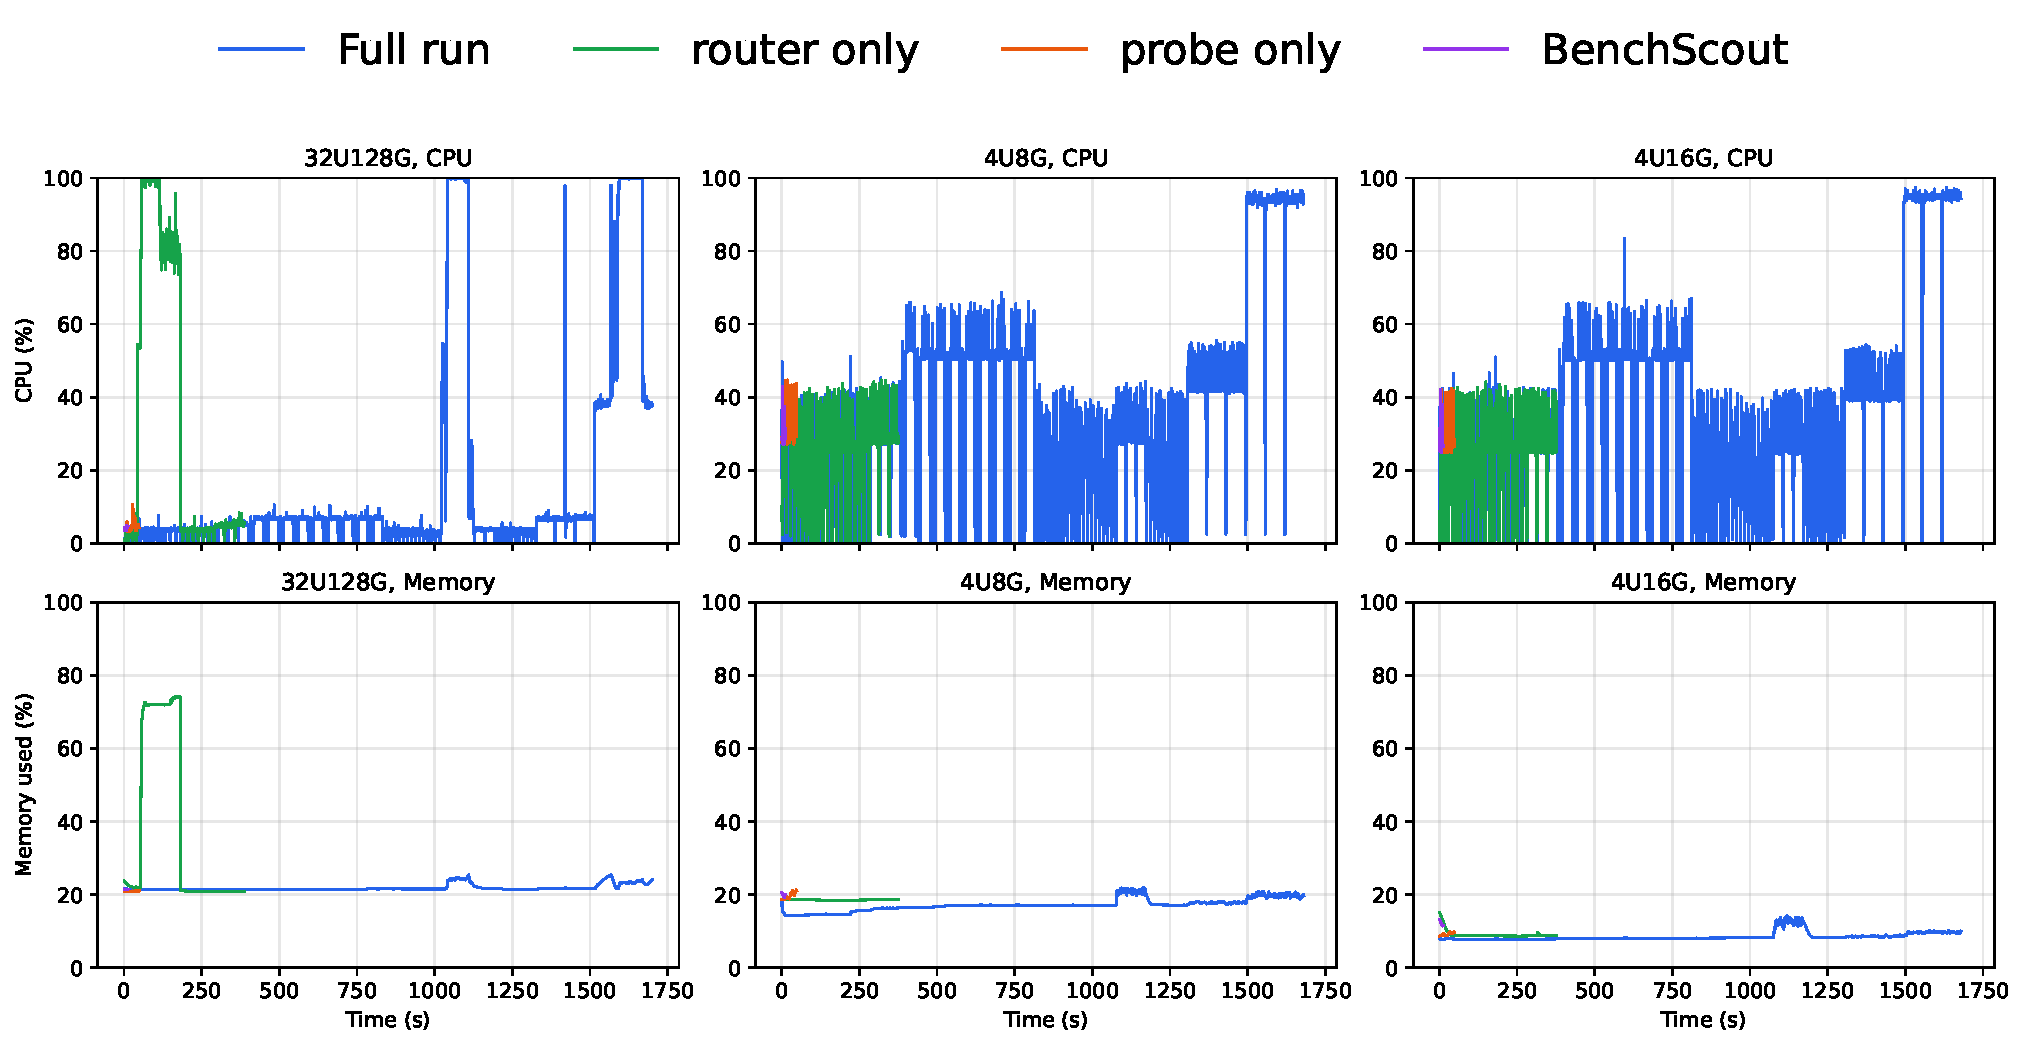
\includegraphics[width=\textwidth]{images/resource_waveforms_2x3.pdf}
    \caption{UnixBench CPU and memory waveforms on H1, H3, and H4 ($0.5$\,s sampling).
    Rows: CPU utilization (\%) and memory used (\%); columns: 32U128G, 4U8G, and 4U16G.
    Curves show \emph{Full run}, \emph{router only}, \emph{probe only}, and \emph{BenchScout} on shared axes (${\approx}1680$\,s horizon).}
    \label{fig:resource-waveforms}
\end{figure*}

\subsection{Model Combination Study}
\label{subsec:model-combination}

The \emph{router only} path isolates the router--reconstructor stack when partial observations are \emph{measured} sub-benchmark scores rather than probe predictions.
We exhaustively evaluate all combinations of three routers (LightGBM, MLP, GNN-expert) and three reconstructors (XGBoost, LightGBM, MLP)---nine combinations per suite on H1---under online partial execution plus reconstruction (the \emph{router only} grid protocol).
Table~\ref{tab:model-combination} reports suite relative error (\%) and benchmark wall-time saved (\%) for each combination; UnixBench uses the H1 grid, with matching H1 grids for \ptscpu{} and \ptsgpu.
Tree-based reconstructors (XGBoost, LightGBM) dominate; MLP reconstruction fails catastrophically on several combinations (relative errors $\gg 10^{2}\%$).

\begin{table}[t]
\centering
\caption{Router--reconstructor combination study on H1 with online partial execution and reconstruction.}
\label{tab:model-combination}
\small
\setlength{\tabcolsep}{3pt}
\begin{tabular}{l|cc|cc|cc}
\toprule
& \multicolumn{6}{c}{\textbf{Reconstructor}} \\
\cmidrule(lr){2-7}
& \multicolumn{2}{c|}{\textbf{XGB}} 
& \multicolumn{2}{c|}{\textbf{LGBM}} 
& \multicolumn{2}{c}{\textbf{MLP}} \\
\cmidrule(lr){2-3} \cmidrule(lr){4-5} \cmidrule(lr){6-7}
\textbf{Router}
& \textbf{Err.} & \textbf{Save} 
& \textbf{Err.} & \textbf{Save} 
& \textbf{Err.} & \textbf{Save} \\
\midrule
\multicolumn{7}{c}{\textit{UnixBench}} \\
\midrule
LightGBM   & 0.926 & 72.5 & 0.619 & 76.3 & 43.8 & 76.5 \\
MLP        & 0.344 & 78.2 & \textbf{0.133} & 72.1 & 42.8 & 79.1 \\
GNN-expert & 0.282 & 76.5 & 0.415 & 76.5 & 59.0 & 76.5 \\
\midrule
\multicolumn{7}{c}{\textit{\ptscpu}} \\
\midrule
LightGBM   & 0.350 & 74.7 & 7.15 & 60.6 & $1.54{\times}10^{4}$ & 80.2 \\
MLP        & 1.30 & 87.5 & \textbf{0.218} & 89.6 & $2.78{\times}10^{3}$ & 92.3 \\
GNN-expert & 3.12 & 95.5 & 3.14 & 39.6 & $1.65{\times}10^{4}$ & 79.5 \\
\midrule
\multicolumn{7}{c}{\textit{\ptsgpu}} \\
\midrule
LightGBM   & 2.03 & 78.0 & \textbf{1.60} & 78.5 & $3.49{\times}10^{2}$ & 78.5 \\
MLP        & 1.61 & 95.3 & 1.61 & 95.3 & $2.83{\times}10^{2}$ & 95.3 \\
GNN-expert & 1.88 & 95.4 & \textbf{1.60} & 94.9 & $4.03{\times}10^{2}$ & 95.3 \\
\bottomrule
\end{tabular}
\end{table}


We identify MLP\,+\,LightGBM reconstruction for UnixBench (0.133\% error) and \ptscpu{} (0.218\%), and LightGBM\,+\,LightGBM for \ptsgpu{} (1.60\%), as the best tree-based \emph{router only} combinations on H1.
The \emph{router only} supplementary studies in Sections~\ref{subsec:topk-tradeoff} and~\ref{subsec:feature-ablation} reuse these best pairs on H1; \emph{probe only} evaluation (Section~\ref{subsec:probe-evaluation}) uses independently trained probe regressors.

\subsection{Probe Model Evaluation}
\label{subsec:probe-evaluation}

This experiment evaluates whether short, time-bounded probes can provide sufficient signal for suite-level performance prediction.
Each component is executed only in micro-probe mode for a fixed budget of 4\,s, optionally collecting eBPF features, and the resulting probe features \(\mathbf{p}_{i,j}\) are used to predict component scores.
Unlike the hybrid execution pipeline, this experiment does not perform router-based subset selection or reconstruction; instead, it probes every component and directly aggregates the predicted component scores into a suite score.

We train two probe regressors, LightGBM and XGBoost, using probe features collected from each host's historical full runs, and evaluate online prediction against the latest full run on the same host.
For PTS suites, labels use \(\log(1+x)\) scaling with per-profile estimators to handle heterogeneous metric magnitudes.
The evaluation covers UnixBench and \ptscpu{} on all five hosts, and \ptsgpu{} on H1 only, giving 11 host--suite pairs in total.

Table~\ref{tab:probe-models} compares LightGBM and XGBoost on H1 across all three suites.
It reports suite relative error, probe wall time \(T_{\mathrm{partial}}\), full-suite wall time \(T_{\mathrm{full}}\) from the ground-truth run JSON, and the resulting wall-time savings.
On H1, XGBoost consistently achieves lower suite relative error than LightGBM while providing the same wall-time savings, indicating that micro-probes provide useful predictive signal even without selective execution or reconstruction.

\begin{table}[t]
\centering
\caption{Probe model comparison on H1.}
\label{tab:probe-models}
\small
\setlength{\tabcolsep}{3pt}
\begin{tabular}{lccccc}
\toprule
\textbf{Suite} & \textbf{Model} & \textbf{Rel.\ err. (\%)} & $T_{\mathrm{partial}}$ (s) & $T_{\mathrm{full}}$ (s) & \textbf{Saved (\%)} \\
\midrule
\multirow{2}{*}{UnixBench}
 & LightGBM & 0.66 & 48.0 & 319.9 & 85.0 \\
 & XGBoost  & 0.45 & 48.0 & 319.9 & 85.0 \\
\midrule
\multirow{2}{*}{\ptscpu}
 & LightGBM & 2.40 & 52.0 & 13018 & 99.6 \\
 & XGBoost  & 1.03 & 52.0 & 13018 & 99.6 \\
\midrule
\multirow{2}{*}{\ptsgpu}
 & LightGBM & 2.60 & 40.0 & 27018 & 99.9 \\
 & XGBoost  & 2.28 & 40.0 & 27018 & 99.9 \\
\bottomrule
\end{tabular}
\end{table}

\subsection{Top-\(K\) Sweep}
\label{subsec:topk-tradeoff}

Using the best \emph{router only} router--reconstructor pairs on H1 from Section~\ref{subsec:model-combination} (MLP\,+\,LightGBM for UnixBench and \ptscpu; LightGBM\,+\,LightGBM for \ptsgpu), we sweep the subset size \(K\) from 1 to 6, capped by the number of components in each suite.
For each \(K\), the router selects Top-\(K\) experts, partial results are observed, and the reconstructor predicts the suite score.
Evaluation uses leave-one-run-out cross-validation on H1's historical runs in the canonical session per suite (random-fold when only one session exists), with router checkpoints and LightGBM reconstructors taken from each session's \id{trained\_models} directory; at each \(K\), the reconstructor is trained with partial subsets of the same size as \(K\).

Figure~\ref{fig:topk-pareto} visualizes the resulting error--saving trade-off, where each point corresponds to one candidate \(K\).
Although the figure does not plot the balanced score directly, the selected \(K\) is determined by minimizing Equation~\ref{eq:balanced-score}, which balances suite relative error against wall-time savings.
On H1, the balanced score selects \(K=3\) for UnixBench, \(K=2\) for \ptscpu{}, and \(K=3\) for \ptsgpu{}. The minimum balanced scores are 1.03 for UnixBench at \(K=3\), 1.01 for \ptscpu{} at \(K=2\), and 1.01 for \ptsgpu{} at \(K=3\).
These choices reflect that suite relative error decreases only modestly as \(K\) grows, while executing additional components quickly reduces wall-time savings.
\ptsgpu{} includes only five GPU-compute profiles in our dataset, so the sweep is capped at \(K=5\).
\begin{figure}
    \centering
    \includegraphics[width=1\linewidth]{images/topk_pareto_tradeoff.pdf}
    \caption{Top-\(K\) error--saving trade-off using the best router--reconstructor pair for each suite.
    Each point corresponds to a candidate \(K\), with numbers indicating \(K\).
    Stars mark the selected \(K\) according to the balanced score in Equation~\ref{eq:balanced-score}.
    Points closer to the lower-right corner achieve lower prediction error and higher time savings.}
    \label{fig:topk-pareto}
\end{figure}

\subsection{System Context Feature Ablation}
\label{subsec:feature-ablation}
To quantify which parts of the system context \(\mathbf{x}\) drive reconstruction accuracy, we ablate feature groups while holding router Top-$K$ selection at $K{=}3$ on H1 (leave-one-run-out CV on each suite's canonical session, random-fold fallback), using the same LightGBM reconstructor and \id{trained\_models} checkpoints as in Section~\ref{subsec:topk-tradeoff}.
We compare four ablated modes against a complete-\(\mathbf{x}\) baseline (not shown):
\id{static\_hw\_only} (hardware topology, memory, cache, and GPU inventory; zero dynamic/PMU),
\id{no\_perf\_pmu} (remove PMU-derived rates except \id{perf\_event\_paranoid}),
\id{no\_dynamic\_proc} (remove load, fault, and bandwidth-proxy dynamics),
and \id{no\_gpu} (remove GPU/OpenCL dimensions).
Table~\ref{tab:feature-ablation} reports mean out-of-fold suite relative error and $\Delta e_m$ (Equation~\ref{eq:xi-importance}) relative to the complete-\(\mathbf{x}\) baseline.
Importance rank (1 = most important to keep among the four ablated groups) sorts ablated modes by descending $\Delta e_m$.
On \ptscpu, ablating static hardware or dynamic \path{/proc} proxies increases error by ${\approx}0.28$~pp; PMU and GPU groups have smaller effects.
On UnixBench all $\Delta e_m$ magnitudes stay below $0.01$~pp on H1.
On \ptsgpu, \id{no\_gpu} yields the largest shift ($\Delta e_m = -0.10$~pp), indicating GPU/OpenCL inventory features most strongly condition reconstruction among the ablated groups.

\begin{table}[t]
\centering
\caption{System-feature ablation at fixed router policy and $K=3$ (offline CV on H1). $\Delta e$ = relative-error change vs.\ complete $\mathbf{x}$ baseline (Equation~\ref{eq:xi-importance}; pp = percentage points; baseline row omitted). Importance rank orders ablated modes by descending $\Delta e$.}
\label{tab:feature-ablation}
\small
\setlength{\tabcolsep}{4pt}
\begin{tabular*}{\columnwidth}{@{\extracolsep{\fill}}l@{\hspace{4pt}}p{0.26\linewidth}ccc@{}}
\toprule
\textbf{Suite} & \textbf{Ablation mode} & \textbf{Rel.\ err. (\%)} & $\Delta e$ (pp) & \textbf{Imp.\ rank} \\
\midrule
\multirow{4}{*}{UnixBench}
 & \id{static\_hw\_only}  & 0.241 & $-$0.003 & 2 \\
 & \id{no\_perf\_pmu}     & 0.243 & 0.000  & 1 \\
 & \id{no\_dynamic\_proc} & 0.241 & $-$0.003 & 3 \\
 & \id{no\_gpu}           & 0.237 & $-$0.007 & 4 \\
\midrule
\multirow{4}{*}{\ptscpu}
 & \id{static\_hw\_only}  & 2.04 & +0.28 & 1 \\
 & \id{no\_perf\_pmu}     & 1.76 & 0.00  & 3 \\
 & \id{no\_dynamic\_proc} & 2.04 & +0.28 & 2 \\
 & \id{no\_gpu}           & 1.75 & $-$0.01 & 4 \\
\midrule
\multirow{4}{*}{\ptsgpu}
 & \id{static\_hw\_only}  & 0.957 & +0.04 & 1 \\
 & \id{no\_perf\_pmu}     & 0.918 & 0.00  & 3 \\
 & \id{no\_dynamic\_proc} & 0.957 & +0.04 & 2 \\
 & \id{no\_gpu}           & 0.818 & $-$0.10 & 4 \\
\bottomrule
\end{tabular*}
\end{table}


\section{Related Work}
\subsection{System Benchmarking and Performance Evaluation}
Benchmarking is a widely used methodology for evaluating the performance of operating systems~\cite{hatt2007benchmarking}. 
A major line of OS benchmarking focuses on measuring low-level operating-system primitives, such as system-call overhead, context switching, process creation, interprocess communication, memory latency, cache behavior, file operations, and network performance. 
Representative microbenchmark suites include LMbench~\cite{brown1997operating}, UnixBench~\cite{smith2011byte}, and HBench-OS~\cite{hatt2007benchmarking}. 
Brown and Seltzer~\cite{brown1997operating} extended the LMbench methodology and introduced HBench-OS to improve benchmarking flexibility, precision, and statistical rigor. 
Beyond performance, Koopman et al.~\cite{koopman1997comparing} proposed a robustness benchmarking method for operating systems using response regions and a CRASH severity scale to characterize erroneous system behavior. 
Kanoun et al.~\cite{kanoun2006dependability} summarized principles and examples of dependability benchmarking, emphasizing reliability, availability, serviceability, and robustness metrics for computer-system evaluation. OS benchmarking has also been adapted to domain-specific operating systems, where evaluation metrics are determined by deployment requirements. 
Garre et al.~\cite{garre2014performance} compared RTOS and GPOS platforms for complex real-time simulations and showed that RTOS platforms can be preferable due to lower IPC and task-switching latency under parallel simulation workloads. 
Watfa et al.~\cite{watfa2014benchmarking} proposed a benchmarking and performance evaluation approach for embedded operating systems in wireless sensor networks, highlighting the tradeoff between event-driven and thread-driven designs. 
Silva et al.~\cite{silva2019operating} benchmarked IoT operating systems such as Contiki-NG, RIOT, and Zephyr using criteria including low-power consumption, real-time capability, security, interoperability, and connectivity. 

\subsection{Performance Prediction}
\label{subsec:rw-performance-prediction}


Simulation-based and statistical modeling methods reduce architectural evaluation cost by simulating only selected configurations and using the results to estimate unexplored design points~\cite{ipek2005approach,ipek2006efficiently,lee2006accurate,sharkawi2009performance}. 
For example, Ipek et al.~\cite{ipek2006efficiently} learned predictive models from sampled architectural simulations to explore large design spaces, while Lee and Brooks~\cite{lee2006accurate} used regression models to predict performance and power from a tiny fraction of simulated microarchitectural configurations. 
Analytical and mechanistic models estimate performance by explicitly modeling processor behavior, such as pipeline effects, cache misses, prefetching, MSHR resources, and execution intervals~\cite{hartstein2002optimum,eyerman2009mechanistic,chen2011hybrid,eyerman2011mechanistic,van2015micro}. 
For instance, Eyerman et al.~\cite{eyerman2009mechanistic} modeled out-of-order execution as intervals separated by disruptive miss events, and Chen and Aamodt~\cite{chen2011hybrid} modeled the performance impact of pending cache hits, prefetching, and limited MSHR resources. 


Machine-learning-based methods have also been widely used to learn complex relationships among programs, hardware characteristics, and performance outcomes. 
Ardalani et al.~\cite{ardalani2015cross} proposed XAPP, which predicts GPU execution time from features of a single-threaded CPU implementation before GPU porting. 
Zheng et al.~\cite{zheng2016accurate} introduced LACross, which predicts phase-level cross-platform performance and power traces from hardware-counter statistics collected on a host platform. 
Wang et al.~\cite{wang2019predicting} used deep neural networks to predict benchmark performance for new CPUs and workloads from public CPU specifications and benchmark datasets. 

\section{Conclusion}

Full-suite system benchmarking remains the gold standard for comparing platforms, yet its all-or-nothing execution model makes repeated measurement impractical in autotuning, multi-machine regression, and production-adjacent monitoring.
We presented \ourmethod, a lightweight pipeline that reframes suite evaluation as conditional expert selection followed by sparse reconstruction.
Motivated by empirical redundancy among UnixBench subtests (Section~\ref{subsec:motivation-redundancy}) and early metric convergence under short runs (Section~\ref{subsec:motivation-convergence}), \ourmethod{} collects a pre-run system context~$\mathbf{x}$, routes to a Top-$K$ subset of informative components, estimates selected scores via time-bounded micro-probes, and reconstructs the full suite profile from partial observations.
The design tolerates imperfect production telemetry---timeouts, missing PMU counters, and disabled eBPF tracing are encoded as features rather than treated as hard failures.

Our evaluation on five heterogeneous Linux hosts (Section~\ref{sec:evaluation}) spans UnixBench and \ptscpu{} on all machines and \ptsgpu{} on a GPU-equipped workstation.
The primary Hybrid path (router $\rightarrow$ probe $\rightarrow$ reconstruct) recovers suite scores with mean relative errors on the order of $10^{-5}$\% while reducing wall time by 95--100\% versus full-suite execution (Table~\ref{tab:overall-effectiveness-expanded}), substantially outperforming execution-free predictors that generalize poorly across hosts.
Resource waveforms confirm that savings come from shorter CPU-active intervals---probe-based paths finish within ${\approx}12$--$48$\,s versus ${\approx}1680$\,s for a full suite---rather than from a substantially lower memory footprint on the 4U8G and 4U16G hosts (Section~\ref{subsec:resource-waveforms}).
\emph{Router only} ablations isolate router--reconstructor choices, Top-$K$ trade-offs, and system-feature groups; \emph{probe only} studies show that probe-based prediction remains sub-percent accurate on H1 across regressor choices (Table~\ref{tab:probe-models}).
Together, these results demonstrate that established suite scores can be approximated with minutes or seconds of observation instead of tens of minutes of full execution, without abandoning the interpretability of standard benchmark indices.

Several directions remain open.
Our models are trained and evaluated per host to respect hardware heterogeneity; cross-host transfer and cold-start routing with fewer historical runs deserve further study.
Hybrid accuracy is computed offline by replaying stored $\mathbf{x}$ and probe telemetry, but partial scores are always probe-model predictions before reconstruction; extending fully live hold-out sessions---where collection and inference occur in one shot without reusing stored $\mathbf{p}$---to additional suites and cloud SKUs would further strengthen deployment claims.
Finally, integrating \ourmethod{} into live autotuning loops---where probe budgets and $K$ must adapt to search progress---is a natural next step toward making comprehensive benchmarking a routine, low-disruption component of systems research and operations.

\bibliographystyle{acm}
\bibliography{sample-base}


\end{document}
\endinput
%%
%% End of file `sample-sigconf.tex'.
